\section{Experiments and results} \label{sec:result}
The experiments mainly include two parts. In the first part, we 
analyze the implementations of the SCGRA overlay based FPGA accelerators with 
different configurations to demonstrate the regularity of the 
SCGRA overlay based FPGA accelerators. In the second part, we benchmark the 
efficiency and quality of the proposed customization framework.

\subsection{Experiment Setup}
All the run time was obtained using a computer with Intel(R) Core(TM) 
i5-3230M CPU and 8GB RAM. Zedboard which has an ARM processor and 
an FPGA was used as the hybrid computation system. Vivado 2013.3 was 
used for the HLS based design and PlanAhead 14.7 was used for the SCGRA overlay based 
design. 

The overlay implementations on Zedboard typically run at 200MHz. We conducted various 
experiments and found that the implementation frequency is almost the same for all the 
different overlay configurations. The power consumption used in this work was 
obtained from XPower which is part of the Xilinx design suite.

\subsection{SCGRA Overlay Implementation Analysis}
In order to analyze the overhead and power of the SCGRA overlay 
based FPGA accelerators, we had three groups of accelerators 
(SCGRA1, SCGRA2, SCGRA3) implemented on Zedboard. The configurations 
are detailed in \tabref{tab:config}. Despite of the diverse 
configurations, all the implementations could meet 200MHz 
timing constrain. With this timing constraint, 
hardware overhead and power consumption are analyzed, which are described 
in the following sub sections.
\begin{table}[tb]
    \tbl{SCGRA Based FPGA Accelerator Configuration \label{tab:config}}{
        \small
        \centering
        \begin{tabular}{c|c|c|c|c|c}
            \hline
            Group & Size & \tabincell{c}{Inst. \\ Rom} & 
            \tabincell{c}{Data \\ Mem} & \tabincell{c}{IBuf \\ /OBuf} & 
            \tabincell{c}{Addr \\Buf} \\ \hline

            SCGRA1 & \tabincell{l}{2x2, 3x2, \\ 3x3, 4x3, \\ 4x4, 5x4} & 
            1kx72 & 256x32 & 2kx32 & 4kx16\\ \hline

            SCGRA2 & \tabincell{l}{2x2, 3x2, \\ 3x3, 4x3, \\4x4} & 
            2kx72 & 256x32 & 2kx32 & 4kx16\\ \hline

            SCGRA3 & \tabincell{l}{2x2, \\ 3x2, \\ 3x3 } &  
            4kx72 & 256x32 & 2kx32 & 4kx16\\ \hline
        \end{tabular}
    }
\end{table}

\subsubsection{Hardware Overhead}
\figref{fig:SCGRA-Overhead} shows the relation between 
the four types of hardware resource overhead and SCGRA 
overlay size. It can be found that FF, LUT and DSP overhead 
do not change much with the memory configurations and they 
present good linearity to the overlay size, thus they can be 
estimated with linear models. BRAM overhead depends 
on both the overlay size and the memory configurations, 
and single variable linear model will not work for the estimation.
Fortunately, it can be calculated precisely with the memory 
configurations. 

\begin{figure}[tb]
    \centering
    \subfloat[\label{fig:FF-Overhead}]{%
      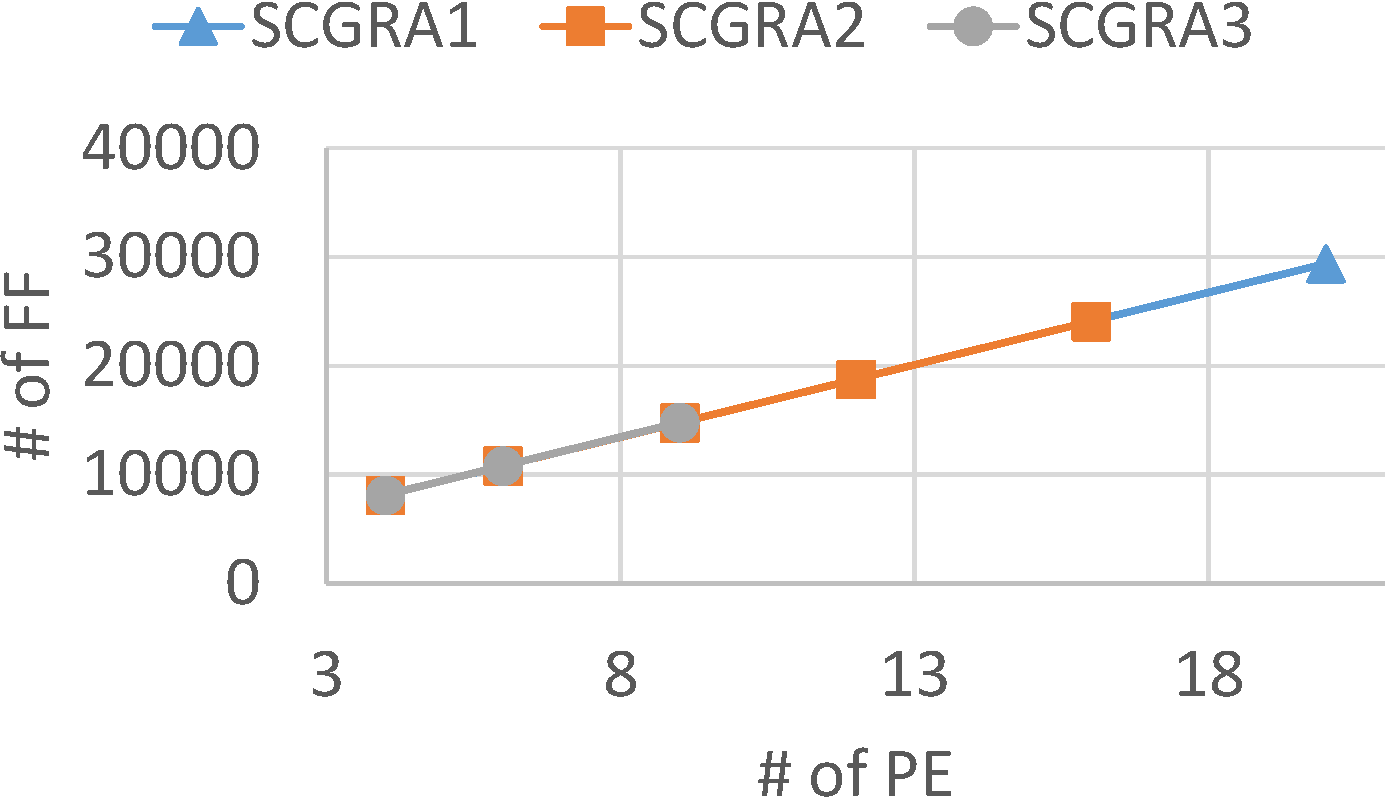
\includegraphics[width=0.35\textwidth]{FF-Overhead}
    }
    \subfloat[\label{fig:LUT-Overhead}]{%
      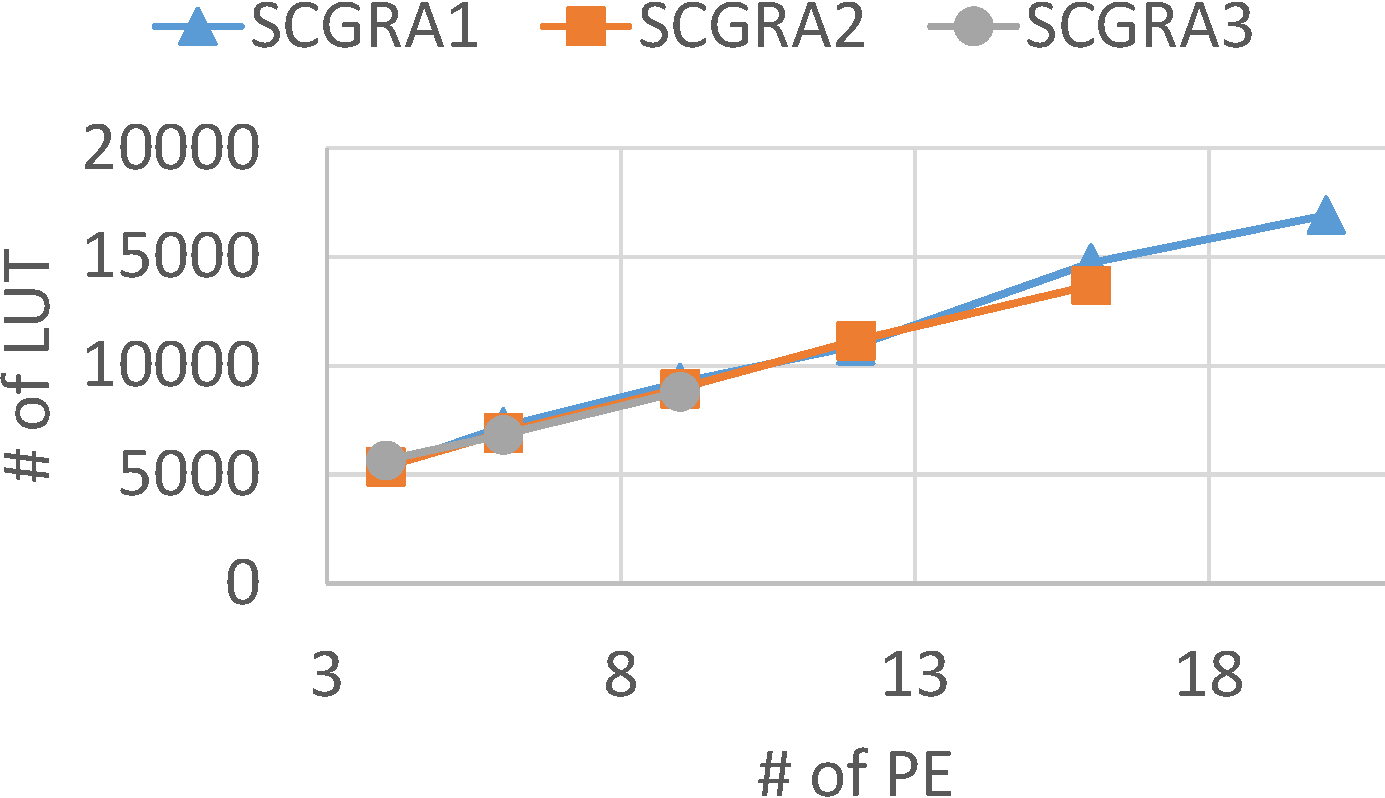
\includegraphics[width=0.35\textwidth]{LUT-Overhead}
    }
    \hfill
    \subfloat[\label{fig:DSP-Overhead}]{%
      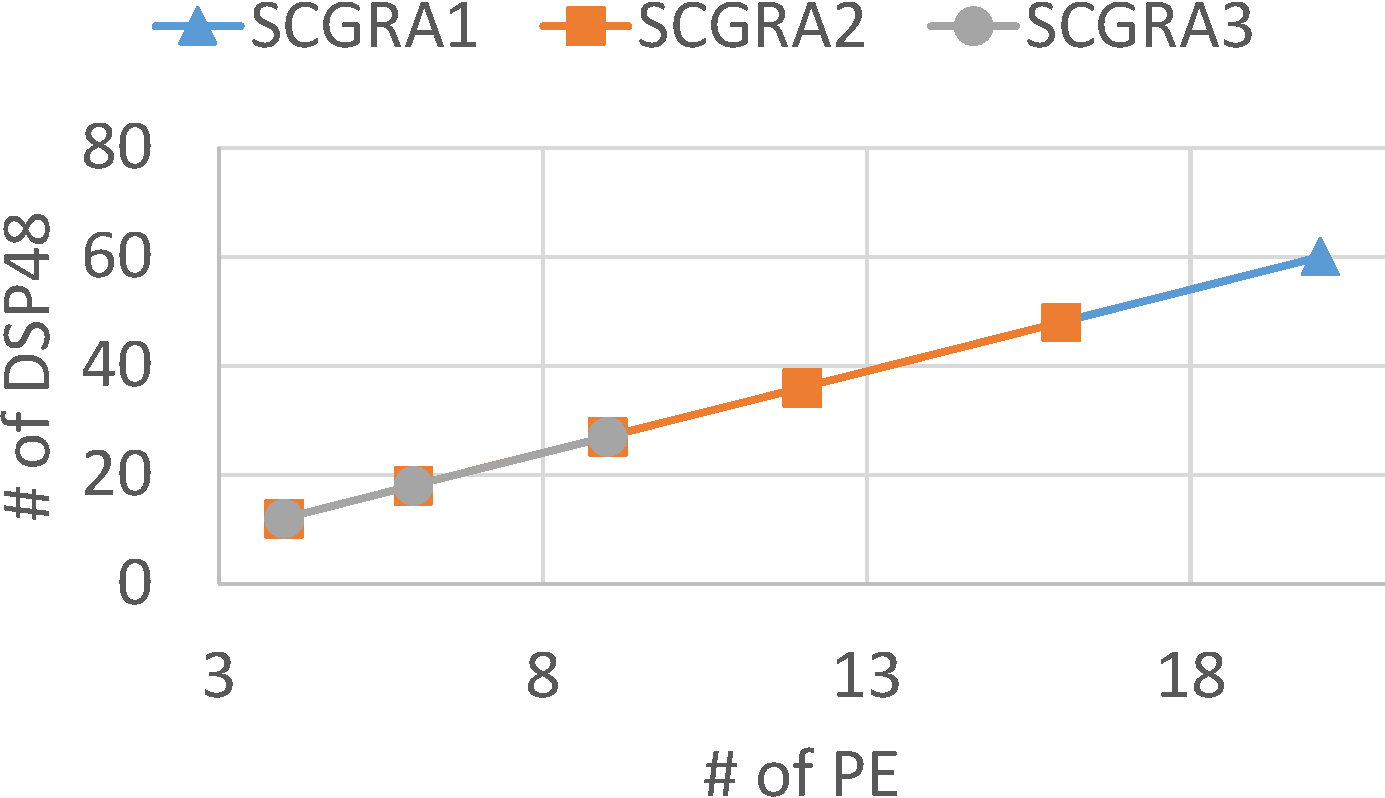
\includegraphics[width=0.35\textwidth]{DSP-Overhead}
    }
    \subfloat[\label{fig:BRAM-Overhead}]{%
      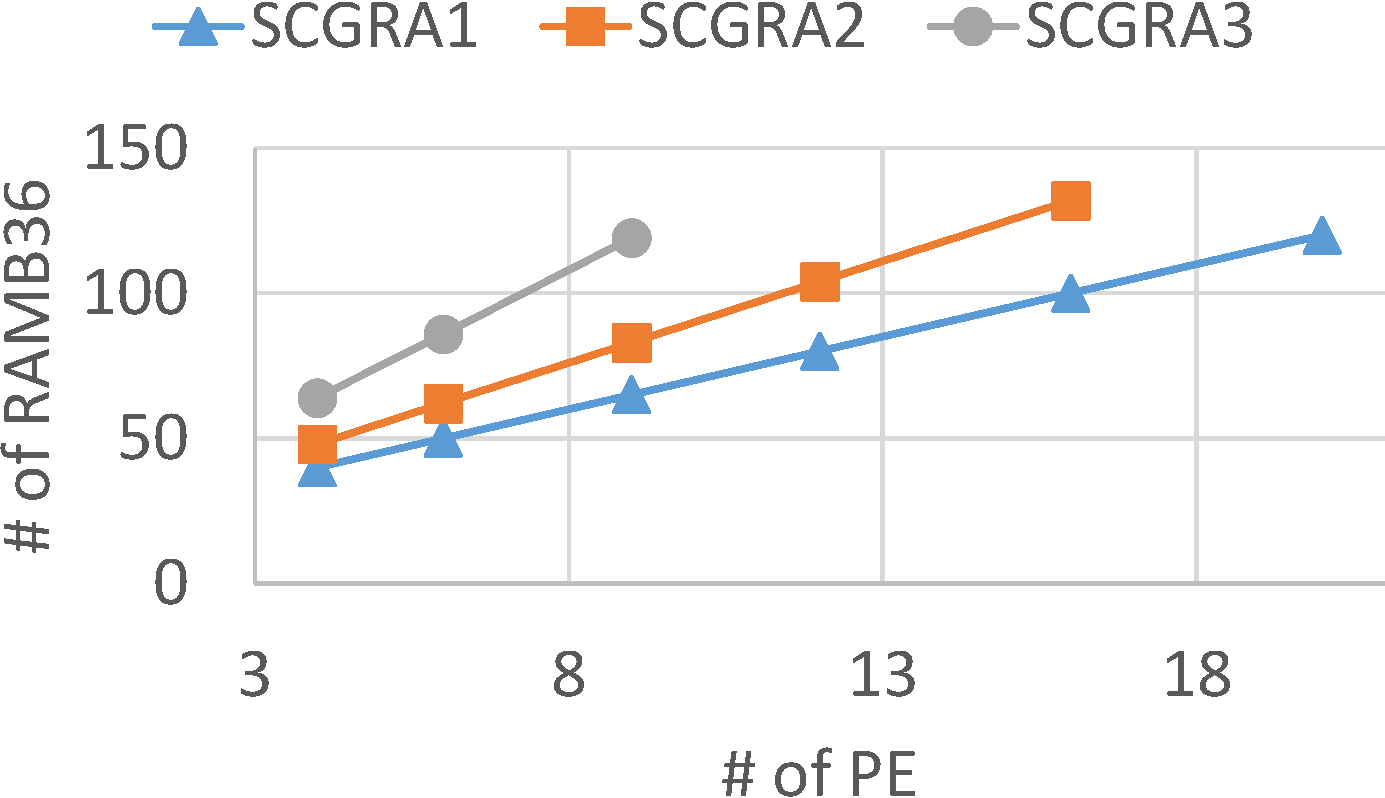
\includegraphics[width=0.35\textwidth]{BRAM-Overhead}
    }
    \caption{Relation between the accelerator overhead and overlay size, 
    (a) FF overhead, (b) LUT overhead, (c)DSP overhead, (d)BRAM overhead}
    \label{fig:SCGRA-Overhead}
\end{figure}


\subsubsection{Power Consumption}
According to the power decomposition in Xpower, the power consumption 
of an FPGA design includes signal power, clock power, BRAM power and so on. 
To simplify the power model of the SCGRA overlay based FPGA accelerator, 
we divide the power consumption into BRAM power and base system 
power which essentially includes the power consumption of the rest part of the system. 
As shown in \figref{fig:SCGRA-Power}, the base system power exhibits good linearity 
over the SCGRA overlay size while the BRAM power is near linear to 
the BRAM overhead. Therefore, both of them can be easily estimated with linear models. 

\begin{figure}[tb]
    \centering
    \subfloat[\label{fig:Base-Power}]{%
      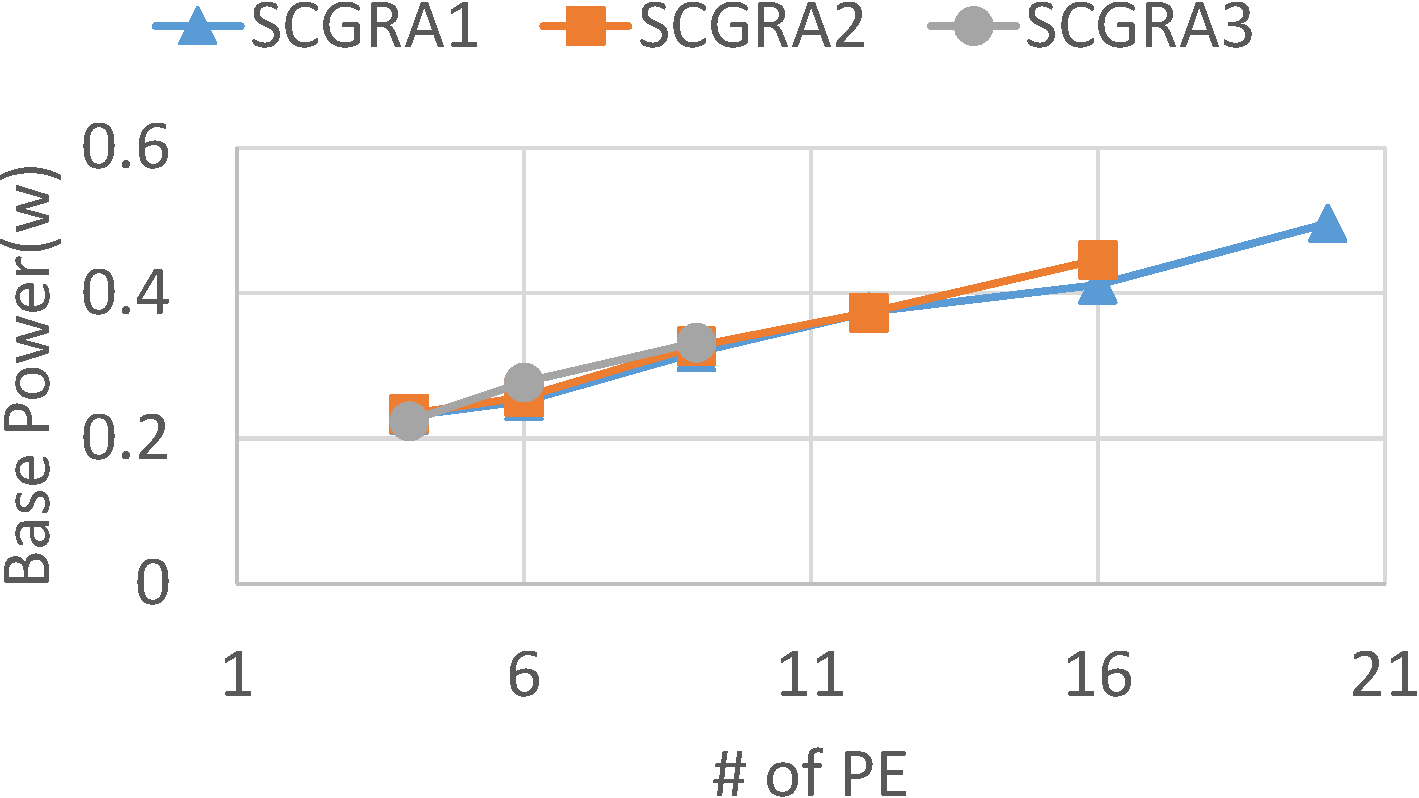
\includegraphics[width=0.35\textwidth]{Base-Power}
    }
    \subfloat[\label{fig:BRAM-Power}]{%
      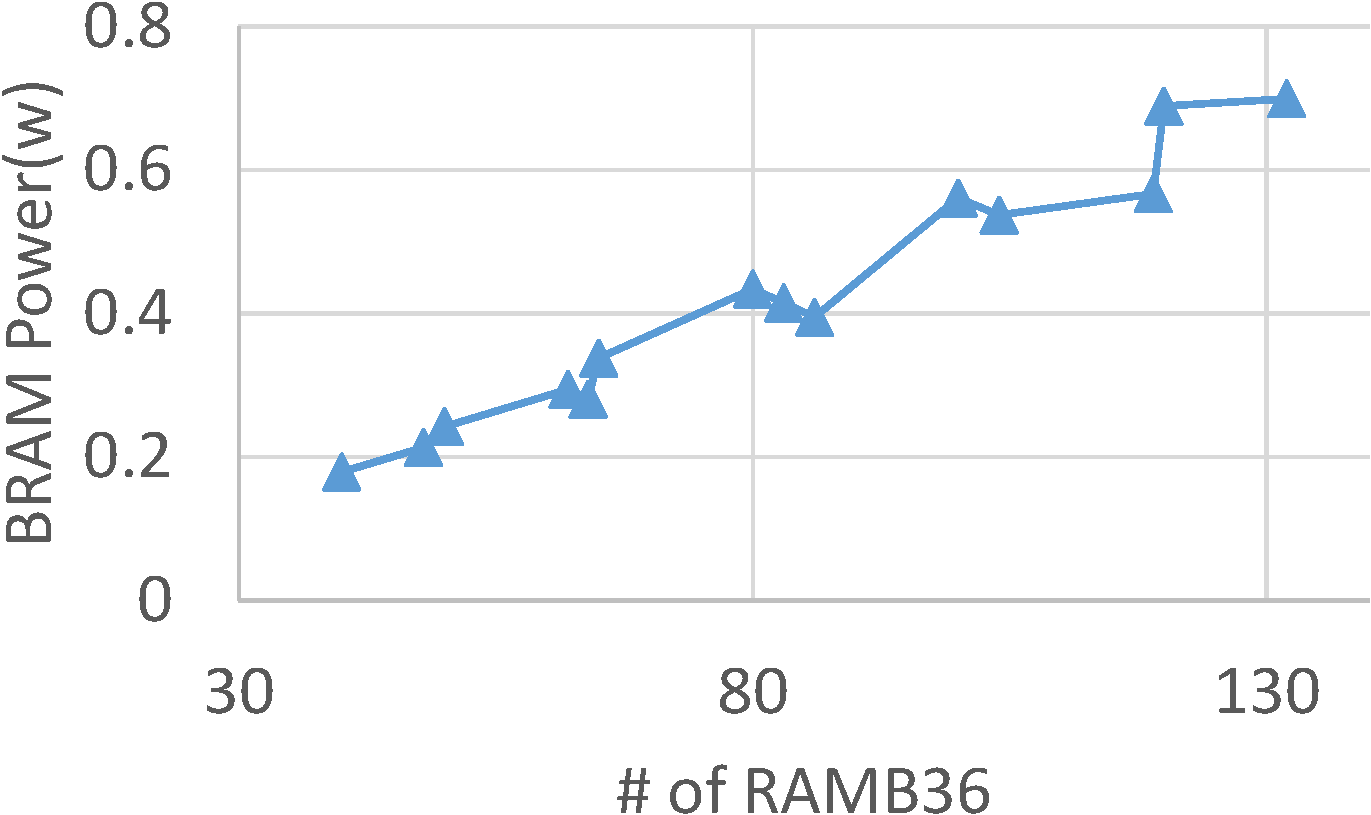
\includegraphics[width=0.35\textwidth]{BRAM-Power}
    }
    \caption{Power consumption of the SCGRA overlay based FPGA accelerator, 
    (a) Base system power including DSP power, clock power, etc., (b) BRAM power}
    \label{fig:SCGRA-Power}
\end{figure}

\subsection{Proposed Design Framework Evaluation}
In this work, we take four applications including Matrix Multiplication (MM), 
FIR, Kmean(KM) and Sobel Edge Detector (SE) as our benchmark. The 
configurations of the benchmark are detailed in \tabref{tab:benchmark-config}. 
In order to evaluate the efficiency and quality of the proposed design 
framework, we implemented the benchmark using both the proposed 
two-step customization (TS) method and an exhaustive search (ES) 
method. Then we compared the Pareto-optimal curves acquired 
using both methods. In addition, we implemented the benchmark 
using Vivado HLS with moderate manual optimization and compared 
the implementations with the ones obtained using the proposed 
customization framework. 
\begin{table}
    \tbl{Benchmark Configurations \label{tab:benchmark-config}}{
        \centering
            \begin{tabular}{l|l|l}
                \hline
                Benchmark & Parameters & Loop Structure \\ \hline
                MM & Matrix Size(128) & $128 \times 128 \times 128$ \\ \hline
                FIR & \tabincell{l}{\# of Input (1024) \\ \# of Taps+1 (64)} & $1024 \times 64$ \\ \hline
                SE & \tabincell{l}{ \# of Vertical Pixels (128) \\ \# of Horizontal Pixels (8)} & $128 \times 8 \times 3 \times 3$ \\ \hline 
                KM & \tabincell{l}{\# of Nodes(1024) \\ \# of Centroids(4) \\ \# of Dimensions(2)} & $1024 \times 4 \times 2$ \\ \hline  
            \end{tabular}

    }
\end{table}


\subsubsection{Customization Methods Comparison}
\figref{fig:DSE-Time} shows the DSE time of both the TS DSE and ES DSE. 
The proposed TS DSE is around 100x faster than the ES DSE on 
average. In particular, ES DSE is extremely slow on MM 
which has three levels of loop with relatively large 
loop count and thus larger design space. Though TS DSE also needs 
longer time to complete the DSE of MM, it skips most 
of the unfeasible configurations and the runtime is 
less sensitive to the size of the design space. 

\begin{figure}[tb]
    \centering
    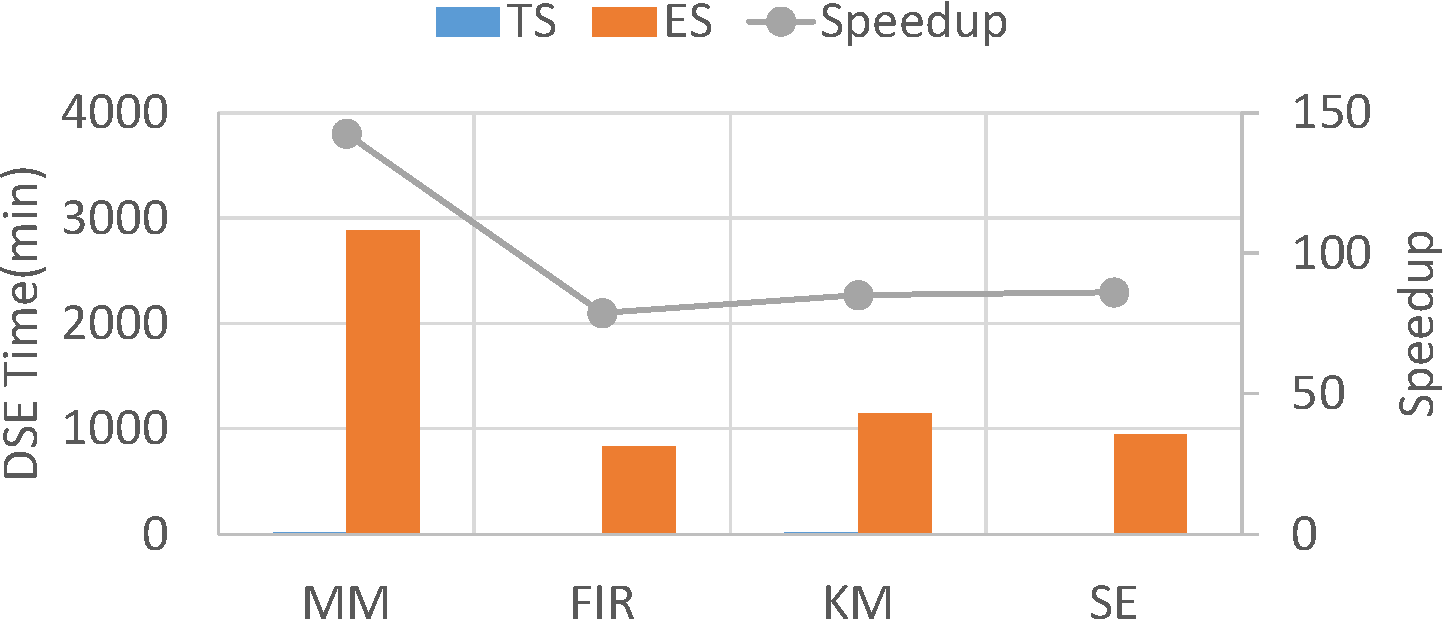
\includegraphics[width=0.45\textwidth]{DSE-Time}
    \caption{DSE time of the benchmark using both TS and ES}
    \label{fig:DSE-Time}
\end{figure}

%\begin{table}[tb]
%    \small
%    \centering
%    \caption{Time Cost for RA DSE and ES DSE\label{tab:dsetime}}{
%        \begin{tabular}{l|l|l|l|l}
%            \hline
%            Benchmark & MM & FIR & KM & SE \\ \hline
%            RA DSE (min) & 20.2 & 10.6 & 13.4 & 11.4\\ \hline
%            ES DSE (min) & 2880.6 & 835.2 & 1140.5 & 946.2\\ \hline
%            Speedup & 142.6 & 78.8 & 85.1 & 86.2 \\ \hline
%        \end{tabular}
%    }
%\end{table}

In order to demonstrate the quality of proposed framework, we presented the 
Pareto-optimal curves acquired from both DSE methods. As shown in \figref{fig:DSE}, 
the Pareto-optimal curves obtained using the two DSE methods are quite 
close to each other. Since TS DSE may prune the design options that involve a larger 
overlay size and better performance according to the sub DSE metric, 
the Pareto-optimal curves may deviate slightly at the higher performance area. 
Fortunately, this can be improved by lowering the user defined metric $\epsilon$ 
while affording longer DSE time. When we customize the design for minimum energy 
consumption, TS DSE achieves the optimal design in all the benchmarks. 

\begin{figure}[tb]
    \centering
	\subfloat[MM]{%
		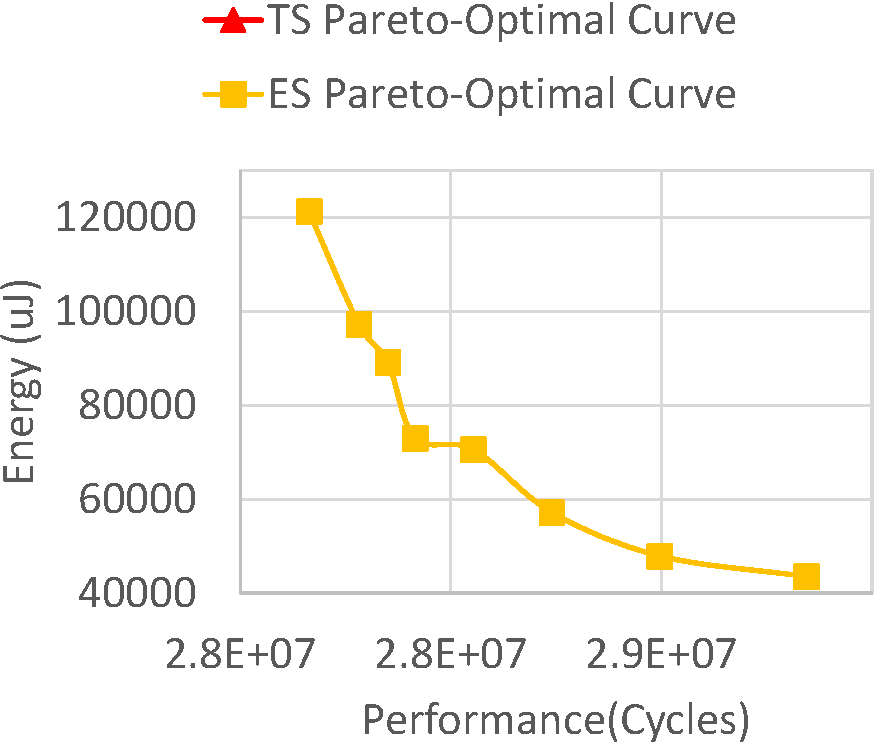
\includegraphics[width=0.35\textwidth]{mm-energy-performance}
	}
	\subfloat[FIR]{%
		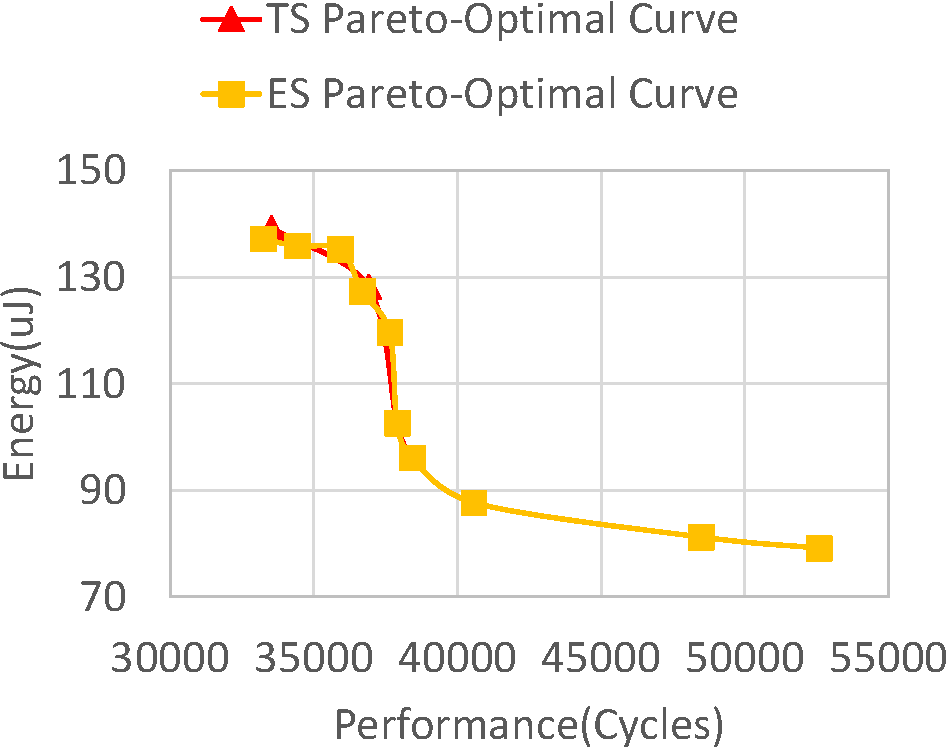
\includegraphics[width=0.35\textwidth]{fir-energy-performance}
	}
    \hfill
	\subfloat[SE]{%
		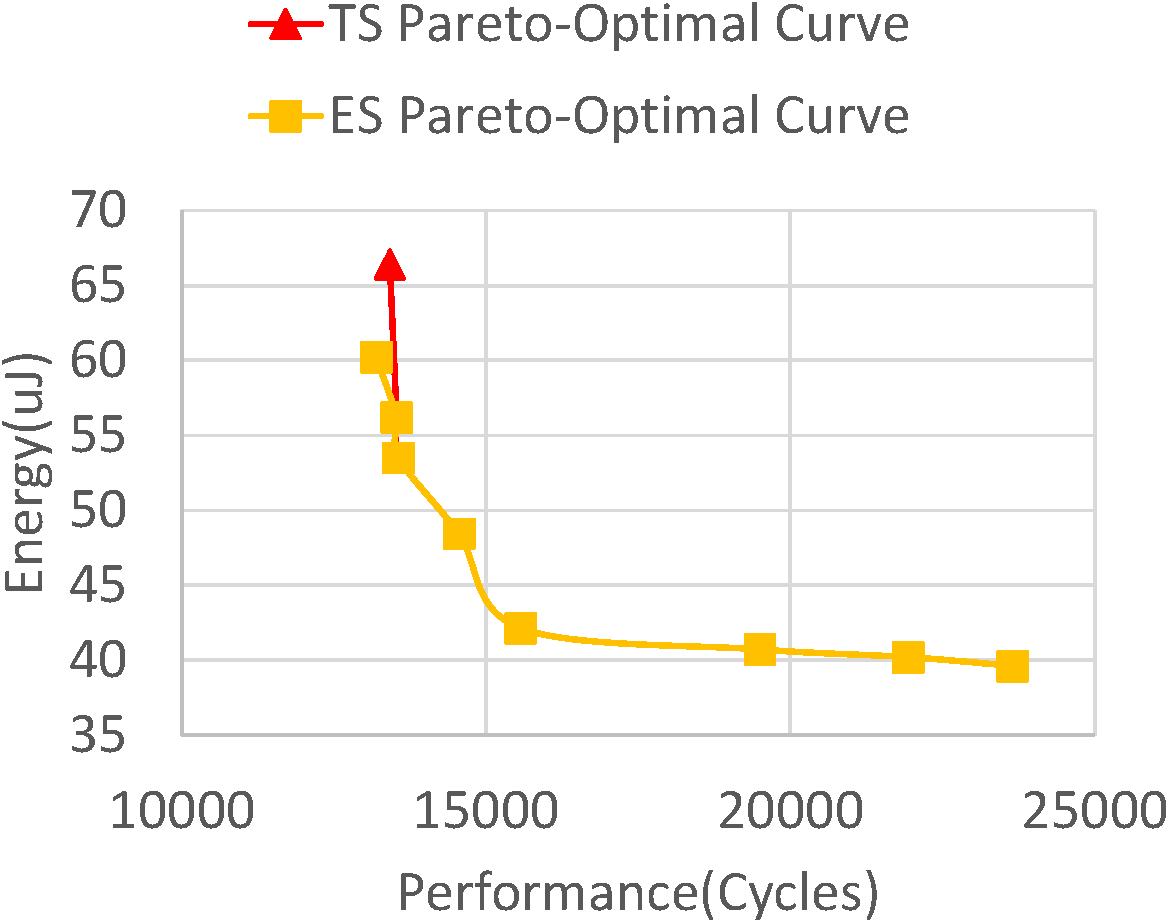
\includegraphics[width=0.35\textwidth]{se-energy-performance}
	}
	\subfloat[KM]{%
		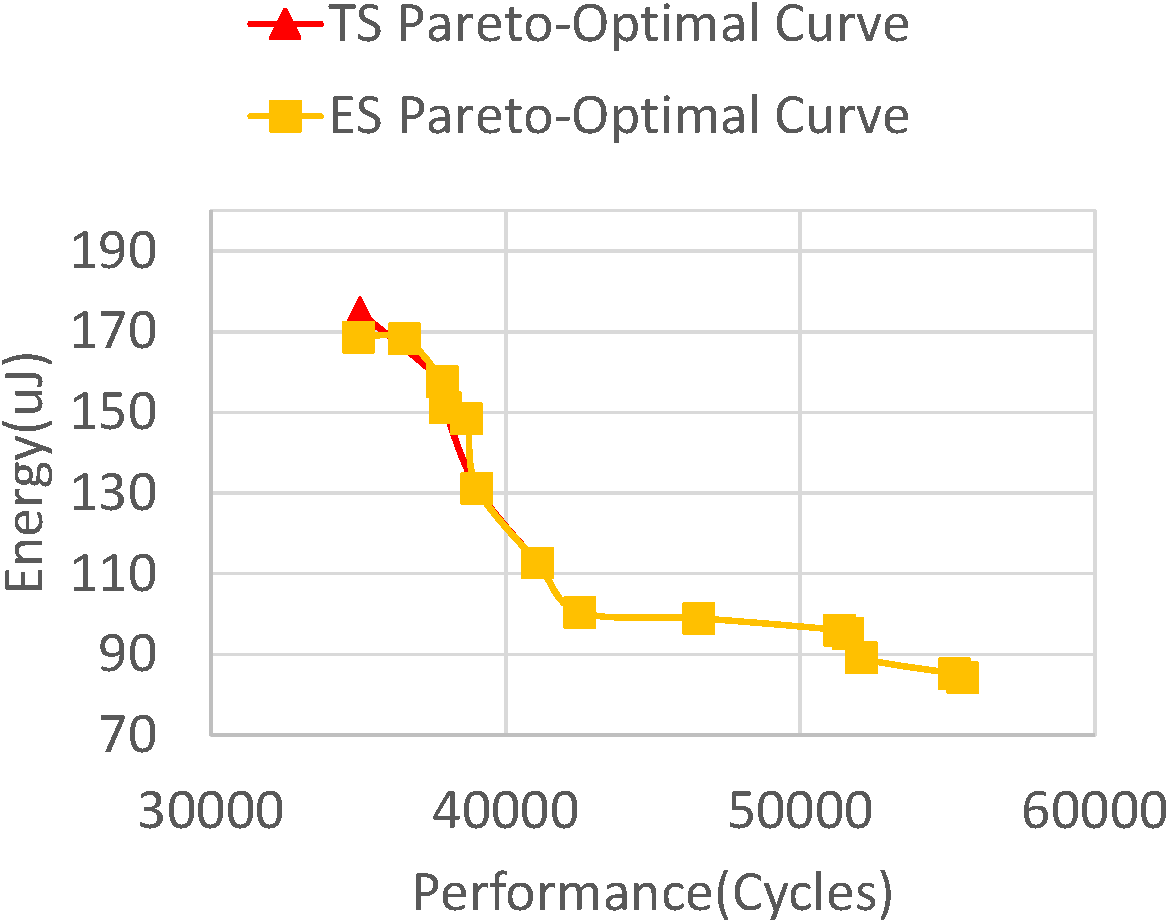
\includegraphics[width=0.35\textwidth]{km-energy-performance}
	}
    \caption{Performance-Energy Pareto-optimal curve}
	\label{fig:DSE}
\end{figure}

\subsubsection{Design Tools Comparison}
The proposed design framework will not be as useful if the performance of the 
generated system is not at least on par with similar systems created with 
conventional HLS tools. For that, we further implemented the 
benchmarks using Vivado HLS with moderate effort. The loops in the benchmark 
were unrolled as much as possible and the input/output buffers were set as large 
as possible. The accelerators generated using HLS run at 100MHz, the accelerators 
built on top of SCGRA overlay have the computation array running at 200MHz 
and the communication fabrics running at 100MHz. Then the accelerators 
generated using both tools were compared. 
Since similar comparison has already been done in previous work \cite{scgra}, 
we just brief the performance comparison for a quick reference.

\begin{figure}[tb]
    \centering
	\subfloat[MM]{%
		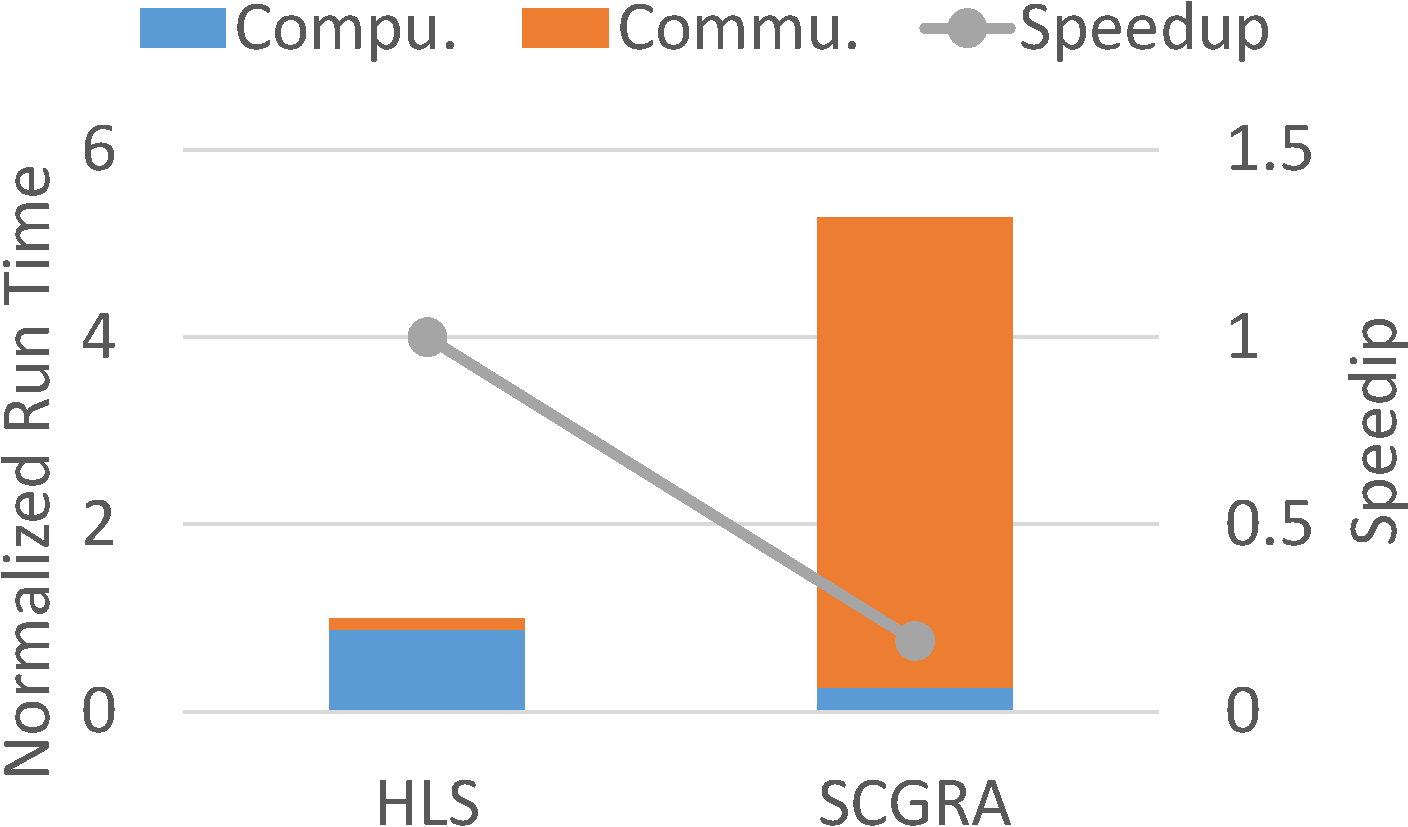
\includegraphics[width=0.35\textwidth]{mm-hls-cp}
	}
	\subfloat[FIR]{%
		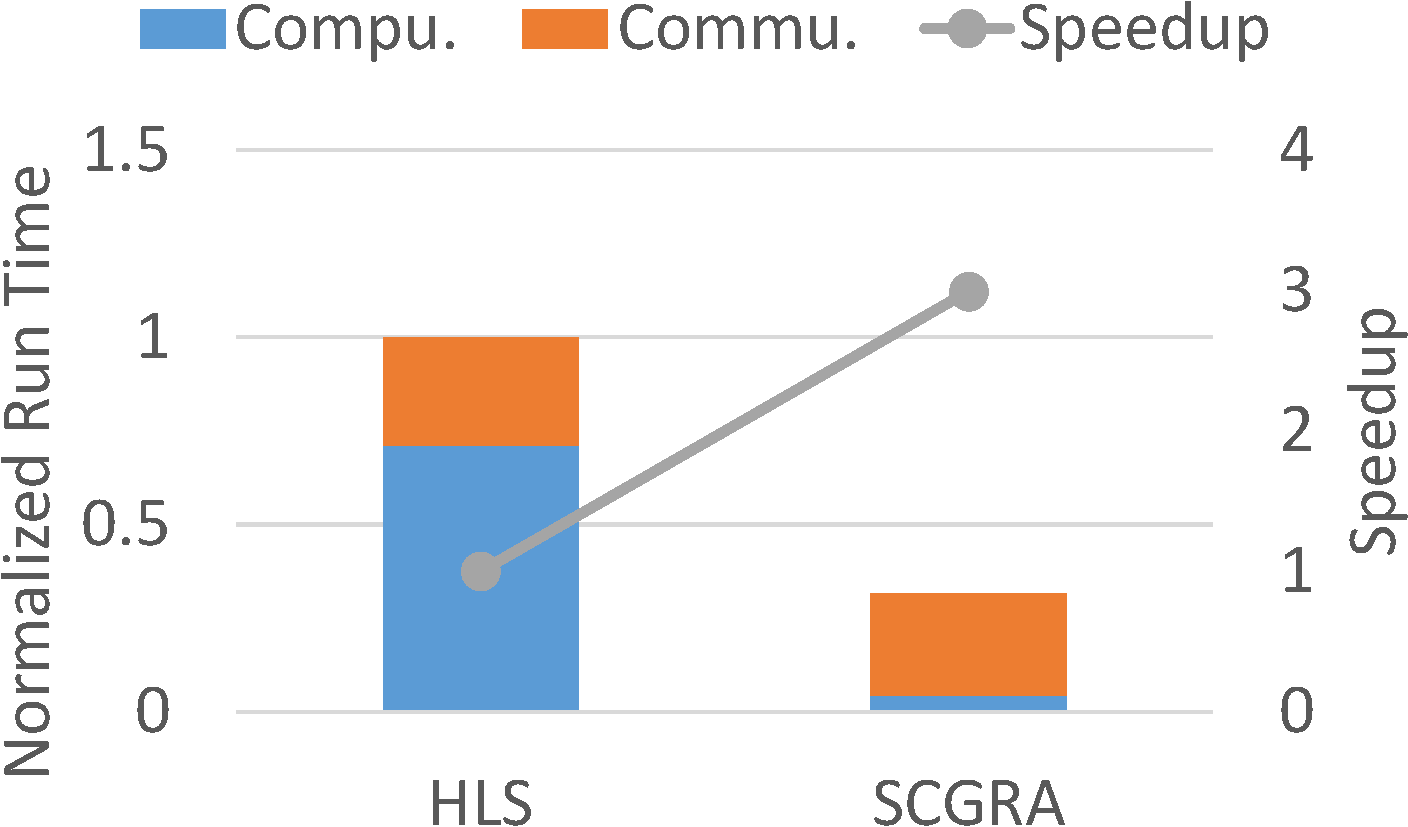
\includegraphics[width=0.35\textwidth]{fir-hls-cp}
	}
    \hfill
	\subfloat[SE]{%
		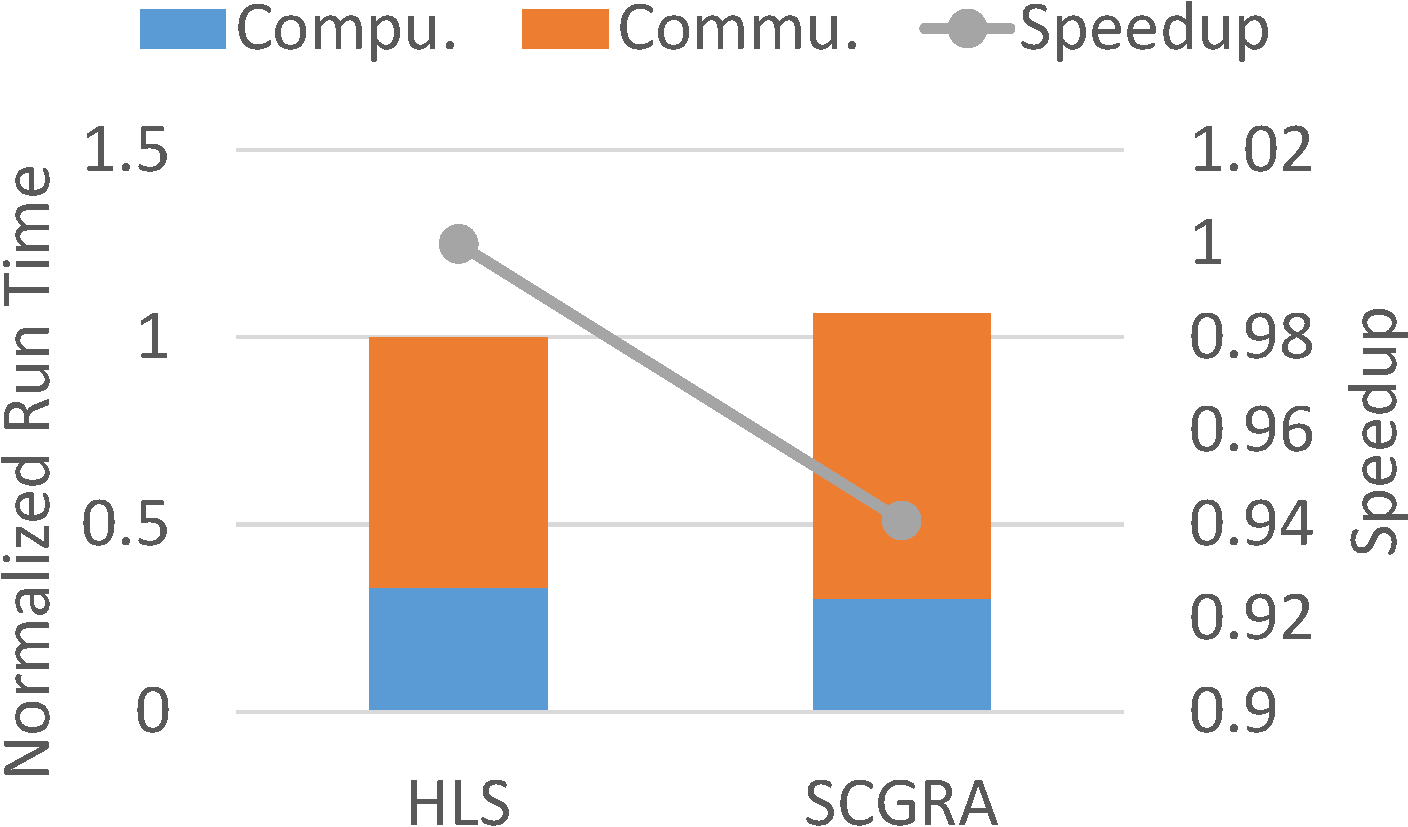
\includegraphics[width=0.35\textwidth]{se-hls-cp}
	}
	\subfloat[KM]{%
		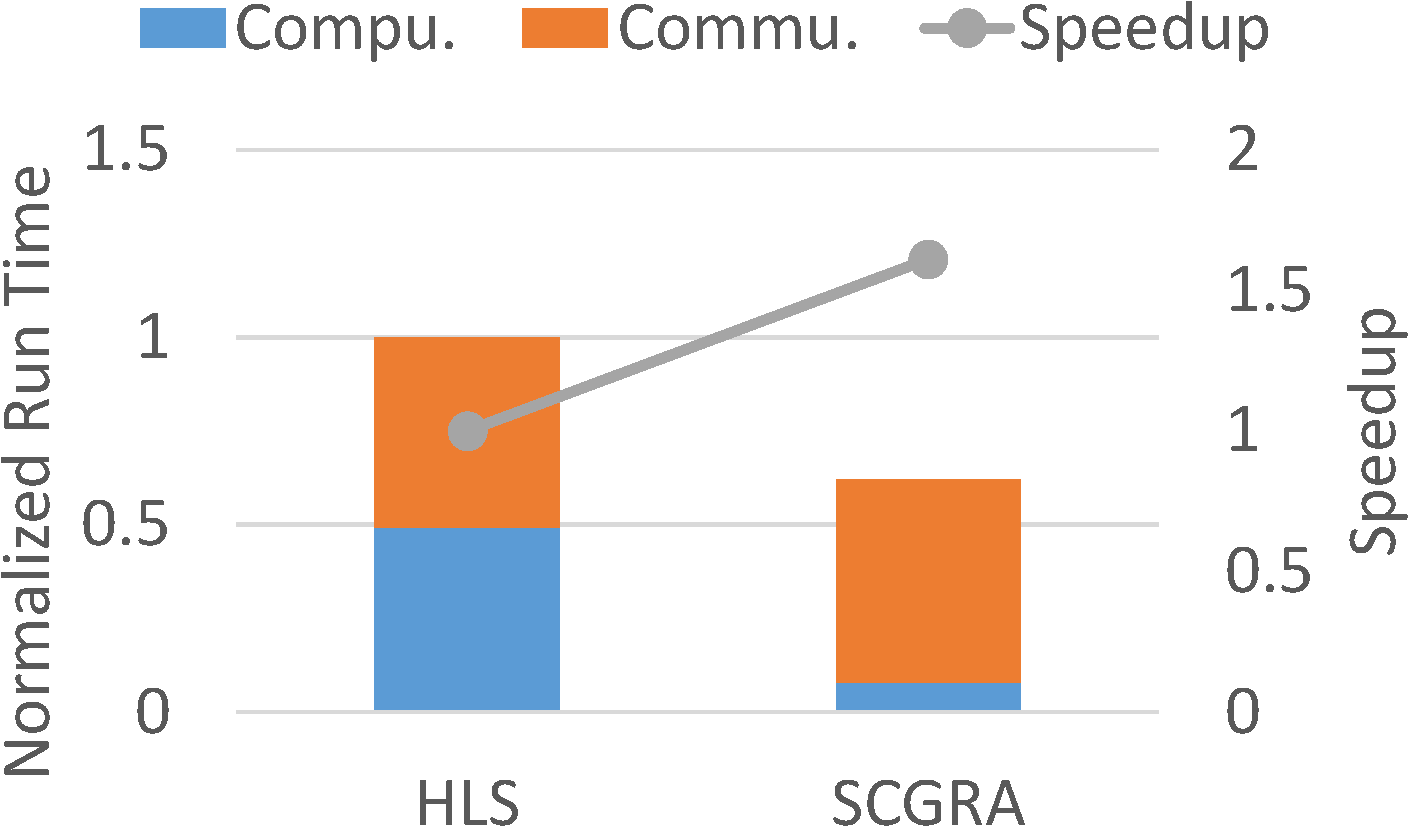
\includegraphics[width=0.35\textwidth]{km-hls-cp}
	}
    \caption{Performance comparison between the implementations 
        using HLS and the proposed automatic customization framework.
    All the run time is normalized to that of the HLS based implementations.}
	\label{fig:hls-cp}
\end{figure}


\figref{fig:hls-cp} shows the performance comparison of the implementations using 
both design tools. The proposed customization framework utilizes 
SCGRA overlay as the backbone and it can't afford large 
BRAM blocks for input/output buffers. As a result, the communication time is larger 
especially when there is a lot of data reuse between consecutive data transmissions.
For instance, HLS based design for MM can afford a 32k-word input buffer storing all 
the input data. However, the SCGRA overlay based design can only 
provide a 4k-word input buffer and it needs to transmit the same data 
multiple times to complete the matrix multiplication (Note that it is 
possible to partly reuse data transmissions of different groups, but it is 
not supported in the experiments). Direct HLS can't support large 
loop unrolling due to the DSP resource constrain. SCGRA overlay based accelerator 
has a lot of distributed intermediate buffers and can accommodate larger loop unrolling.
Therefore, the accelerators generated using the proposed framework provides competitive 
pure computation time and overall performance especially for compute intensive loops.


